% Created by tikzDevice version 0.12.3.1 on 2022-09-01 15:57:45
% !TEX encoding = UTF-8 Unicode
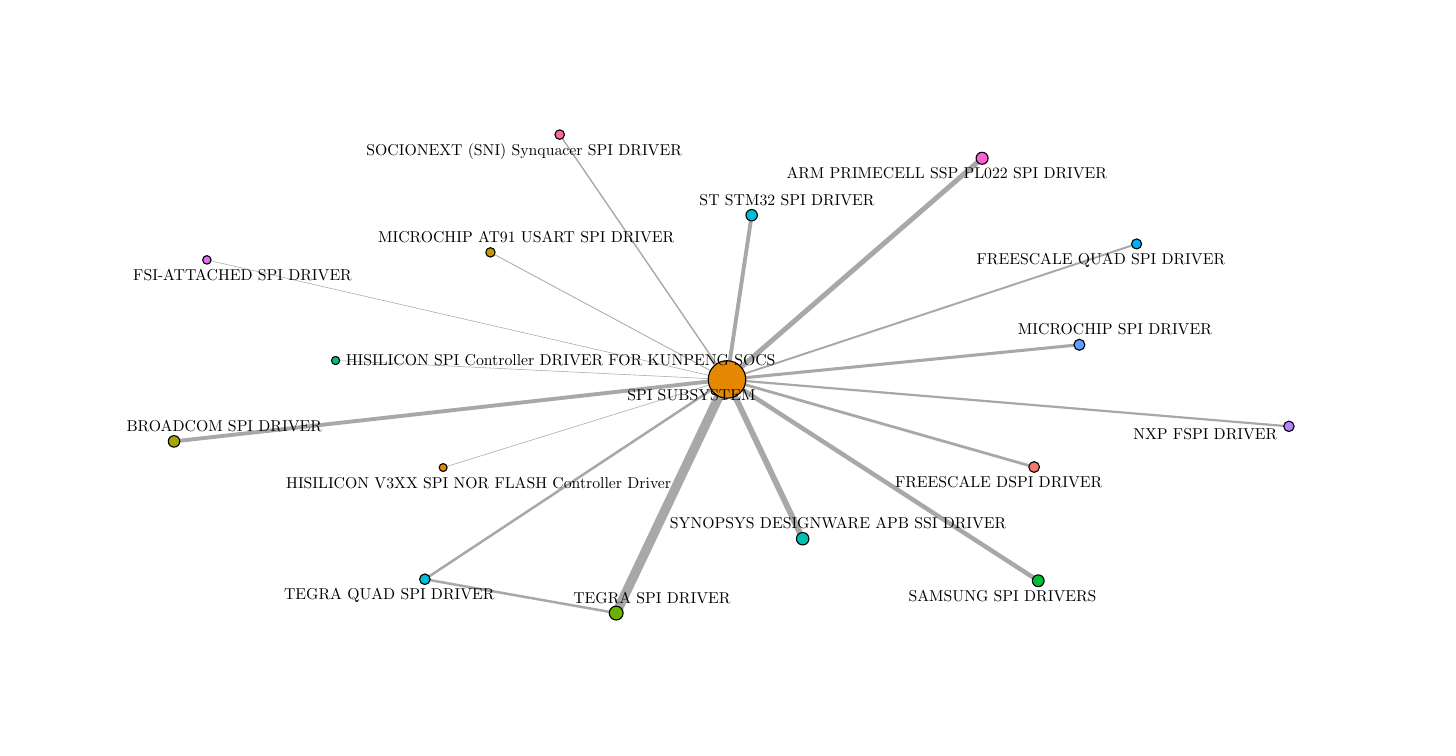
\begin{tikzpicture}[x=1pt,y=1pt]
\definecolor{fillColor}{RGB}{255,255,255}
\path[use as bounding box,fill=fillColor,fill opacity=0.00] (0,0) rectangle (505.89,252.94);
\begin{scope}
\path[clip] (  0.00,  0.00) rectangle (505.89,252.94);
\definecolor{fillColor}{RGB}{255,255,255}

\path[fill=fillColor] (  0.00,  0.00) rectangle (505.89,252.94);
\end{scope}
\begin{scope}
\path[clip] ( 32.75, 32.75) rectangle (475.89,222.94);
\definecolor{drawColor}{gray}{0.66}

\path[draw=drawColor,line width= 1.8pt,line join=round] (344.88,205.75) -- (252.70,125.81);

\path[draw=drawColor,line width= 1.4pt,line join=round] ( 52.89,103.44) -- (252.70,125.81);

\path[draw=drawColor,line width= 1.0pt,line join=round] (363.68, 94.18) -- (252.70,125.81);

\path[draw=drawColor,line width= 0.7pt,line join=round] (400.70,174.79) -- (252.70,125.81);

\path[draw=drawColor,line width= 0.2pt,line join=round] ( 64.75,169.02) -- (252.70,125.81);

\path[draw=drawColor,line width= 0.2pt,line join=round] (111.26,132.67) -- (252.70,125.81);

\path[draw=drawColor,line width= 0.2pt,line join=round] (150.13, 93.99) -- (252.70,125.81);

\path[draw=drawColor,line width= 0.3pt,line join=round] (167.22,171.75) -- (252.70,125.81);

\path[draw=drawColor,line width= 1.1pt,line join=round] (380.04,138.36) -- (252.70,125.81);

\path[draw=drawColor,line width= 0.8pt,line join=round] (455.75,108.88) -- (252.70,125.81);

\path[draw=drawColor,line width= 1.6pt,line join=round] (365.17, 53.08) -- (252.70,125.81);

\path[draw=drawColor,line width= 0.5pt,line join=round] (192.24,214.30) -- (252.70,125.81);

\path[draw=drawColor,line width= 1.4pt,line join=round] (252.70,125.81) -- (261.61,185.17);

\path[draw=drawColor,line width= 2.1pt,line join=round] (252.70,125.81) -- (280.04, 68.27);

\path[draw=drawColor,line width= 0.9pt,line join=round] (252.70,125.81) -- (143.52, 53.63);

\path[draw=drawColor,line width= 3.4pt,line join=round] (252.70,125.81) -- (212.66, 41.40);

\path[draw=drawColor,line width= 0.9pt,line join=round] (143.52, 53.63) -- (212.66, 41.40);
\definecolor{drawColor}{RGB}{0,0,0}
\definecolor{fillColor}{RGB}{253,97,209}

\path[draw=drawColor,line width= 0.4pt,line join=round,line cap=round,fill=fillColor] (344.88,205.75) circle (  2.17);
\definecolor{fillColor}{RGB}{163,165,0}

\path[draw=drawColor,line width= 0.4pt,line join=round,line cap=round,fill=fillColor] ( 52.89,103.44) circle (  2.07);
\definecolor{fillColor}{RGB}{248,118,109}

\path[draw=drawColor,line width= 0.4pt,line join=round,line cap=round,fill=fillColor] (363.68, 94.18) circle (  1.94);
\definecolor{fillColor}{RGB}{0,176,246}

\path[draw=drawColor,line width= 0.4pt,line join=round,line cap=round,fill=fillColor] (400.70,174.79) circle (  1.82);
\definecolor{fillColor}{RGB}{231,107,243}

\path[draw=drawColor,line width= 0.4pt,line join=round,line cap=round,fill=fillColor] ( 64.75,169.02) circle (  1.53);
\definecolor{fillColor}{RGB}{0,191,125}

\path[draw=drawColor,line width= 0.4pt,line join=round,line cap=round,fill=fillColor] (111.26,132.67) circle (  1.48);
\definecolor{fillColor}{RGB}{229,135,0}

\path[draw=drawColor,line width= 0.4pt,line join=round,line cap=round,fill=fillColor] (150.13, 93.99) circle (  1.43);
\definecolor{fillColor}{RGB}{201,152,0}

\path[draw=drawColor,line width= 0.4pt,line join=round,line cap=round,fill=fillColor] (167.22,171.75) circle (  1.69);
\definecolor{fillColor}{RGB}{97,156,255}

\path[draw=drawColor,line width= 0.4pt,line join=round,line cap=round,fill=fillColor] (380.04,138.36) circle (  1.99);
\definecolor{fillColor}{RGB}{185,131,255}

\path[draw=drawColor,line width= 0.4pt,line join=round,line cap=round,fill=fillColor] (455.75,108.88) circle (  1.88);
\definecolor{fillColor}{RGB}{0,186,56}

\path[draw=drawColor,line width= 0.4pt,line join=round,line cap=round,fill=fillColor] (365.17, 53.08) circle (  2.13);
\definecolor{fillColor}{RGB}{255,103,164}

\path[draw=drawColor,line width= 0.4pt,line join=round,line cap=round,fill=fillColor] (192.24,214.30) circle (  1.72);
\definecolor{fillColor}{RGB}{229,135,0}

\path[draw=drawColor,line width= 0.4pt,line join=round,line cap=round,fill=fillColor] (252.70,125.81) circle (  6.78);
\definecolor{fillColor}{RGB}{0,188,216}

\path[draw=drawColor,line width= 0.4pt,line join=round,line cap=round,fill=fillColor] (261.61,185.17) circle (  2.06);
\definecolor{fillColor}{RGB}{0,192,175}

\path[draw=drawColor,line width= 0.4pt,line join=round,line cap=round,fill=fillColor] (280.04, 68.27) circle (  2.25);
\definecolor{fillColor}{RGB}{0,188,216}

\path[draw=drawColor,line width= 0.4pt,line join=round,line cap=round,fill=fillColor] (143.52, 53.63) circle (  1.91);
\definecolor{fillColor}{RGB}{107,177,0}

\path[draw=drawColor,line width= 0.4pt,line join=round,line cap=round,fill=fillColor] (212.66, 41.40) circle (  2.50);

\node[text=drawColor,anchor=base,inner sep=0pt, outer sep=0pt, scale=  0.57] at (332.12,198.28) {ARM PRIMECELL SSP PL022 SPI DRIVER};

\node[text=drawColor,anchor=base,inner sep=0pt, outer sep=0pt, scale=  0.57] at ( 71.04,107.01) {BROADCOM SPI DRIVER};

\node[text=drawColor,anchor=base,inner sep=0pt, outer sep=0pt, scale=  0.57] at (350.86, 86.71) {FREESCALE DSPI DRIVER};

\node[text=drawColor,anchor=base,inner sep=0pt, outer sep=0pt, scale=  0.57] at (387.81,167.31) {FREESCALE QUAD SPI DRIVER};

\node[text=drawColor,anchor=base,inner sep=0pt, outer sep=0pt, scale=  0.57] at ( 77.64,161.52) {FSI-ATTACHED SPI DRIVER};

\node[text=drawColor,anchor=base,inner sep=0pt, outer sep=0pt, scale=  0.57] at (192.61,130.86) {HISILICON SPI Controller DRIVER FOR KUNPENG SOCS};

\node[text=drawColor,anchor=base,inner sep=0pt, outer sep=0pt, scale=  0.57] at (162.96, 86.52) {HISILICON V3XX SPI NOR FLASH Controller Driver};

\node[text=drawColor,anchor=base,inner sep=0pt, outer sep=0pt, scale=  0.57] at (180.15,175.32) {MICROCHIP AT91 USART SPI DRIVER};

\node[text=drawColor,anchor=base,inner sep=0pt, outer sep=0pt, scale=  0.57] at (392.88,141.93) {MICROCHIP SPI DRIVER};

\node[text=drawColor,anchor=base,inner sep=0pt, outer sep=0pt, scale=  0.57] at (425.53,104.12) {NXP FSPI DRIVER};

\node[text=drawColor,anchor=base,inner sep=0pt, outer sep=0pt, scale=  0.57] at (352.27, 45.60) {SAMSUNG SPI DRIVERS};

\node[text=drawColor,anchor=base,inner sep=0pt, outer sep=0pt, scale=  0.57] at (179.40,206.82) {SOCIONEXT (SNI) Synquacer SPI DRIVER};

\node[text=drawColor,anchor=base,inner sep=0pt, outer sep=0pt, scale=  0.57] at (239.83,118.34) {SPI SUBSYSTEM};

\node[text=drawColor,anchor=base,inner sep=0pt, outer sep=0pt, scale=  0.57] at (274.39,188.72) {ST STM32 SPI DRIVER};

\node[text=drawColor,anchor=base,inner sep=0pt, outer sep=0pt, scale=  0.57] at (292.86, 71.82) {SYNOPSYS DESIGNWARE APB SSI DRIVER};

\node[text=drawColor,anchor=base,inner sep=0pt, outer sep=0pt, scale=  0.57] at (130.67, 46.15) {TEGRA QUAD SPI DRIVER};

\node[text=drawColor,anchor=base,inner sep=0pt, outer sep=0pt, scale=  0.57] at (225.55, 44.96) {TEGRA SPI DRIVER};
\end{scope}
\end{tikzpicture}
